\definecolor{cfwone}{HTML}{eef5fa}
\definecolor{cfwtwo}{HTML}{daeaf5}
\definecolor{cfwthree}{HTML}{b2d2e9}
\definecolor{cfwfour}{HTML}{8abbde}

\newcommand{\fwone}[1]{\colbox{cfwone}{#1}\xspace}
\newcommand{\fwtwo}[1]{\colbox{cfwtwo}{#1}\xspace}
\newcommand{\fwthree}[1]{\colbox{cfwthree}{#1}\xspace}
\newcommand{\fwfour}[1]{\colbox{cfwfour}{#1}\xspace}

\newcommand{\fexp}[2]{\texttt{[{\color{darkgray}{#1:#2}}]}\xspace}
\newcommand{\fexptag}[1]{\fexp{TAG}{#1}}
\newcommand{\fexpfrom}[1]{\fexp{FROM}{#1}}
\newcommand{\fexpto}[1]{\fexp{TO}{#1}}
\newcommand{\fexptemp}[1]{\fexp{TEMP}{#1}}


\section{Counterfactual Explanations}

%Both counterfactual explanations and semi-counterfactual explanations.
%As defined in \cite{}

\subsection{Local explanations: Abnormality}





\begin{figure}[t]
\centering
\includegraphics[trim={0 18cm 31cm 0cm},clip,width=1\columnwidth]{figures/explanation_v2}
\vspace{-15pt}
\caption{
Counterfactual explanations on a \qqp instance (A), which compensates the feature weights from SHAP visualized by the blue backgrounds and the bar chart.
Counterfactuals can 
(B) concretize the opaque weights using readable examples. so it is more noticeable that the model does not recognize ``reasons'';
(C) alert errors missed by SHAP, so users are not misled to believe that the model will respond correctly to changed person names.
\wts{Somewhere in the text: highlight (B)?}
}
\vspace{-10pt}
\label{fig:explanation}
\end{figure}

%\wts{Finding bugs missed by the feature attribution, and concretizing the opaque weights using readable examples.}
Compared to feature attribution methods, counterfactual explanations more naturally answer users' 

The cognitive burden of complete explanations is too great.
As a result, \citet{miller} concluded that people usually \emph{select} a small subset of (counterfactual) explanations on contrastive cases (``foils'') that they find unexpected. 
As such, he further proposed that ``abnormality could be used to infer likely foils.''
Here, we operationalize the concept of abnormality based on \emph{the discrepancy between the expected and the actual changes in the prediction}, and use it as our selection method.

Given a prediction model $f$, we define the actual change in prediction as $d_f(\xp, x)$, and the expected prediction change as $\hat{d}_f(\xp, x)$.
The distance between the expectation and reality then becomes:
$$\Delta d_f(\xp, x) = |\hat{d}_f(\xp, x)-d_f(\xp, x)|$$
We select two abnormal, ``turning point'' counterfactuals, \ie unexpected large changes in prediction when small (large) change is expected:
$$ \xp_a^1 = \argmax_{\xp} \Delta d_f(\xp, x), \xp_a^2 = \argmin_{\xp} \Delta d_f(\xp, x)$$
Whereas $d_f(\xp, x)=|f_p(\xp)-f_p(x)|$ where $f(x)$ denotes the prediction probability of $f$ on $x$, $d_f(\xp, x)$ can take various forms. 
As a standalone explanation method, it can be the cosine distance in the \emph{Embedding space}.
The embedding can be either model-agnostic (\eg with~sentence transformers~\cite{reimers-2019-sentence-bert}), or the last layer of the hidden state of the finetuned predictor.

On the other hand, as a \emph{compensation} to existing feature attribution methods, $\hat{d}_f$ can be the importance (weights) of the perturbed tokens in $x$, estimated by feature attribution methods.
As mentioned in \S\ref{sec:relate}, methods like SHAP or LIME only estimate feature weights by \emph{masking} the words, which do not represent how model would react in non-deletion counterfactuals (replacing words or inserting negations).
Therefore, abnormalities selected in this way can  compensate or criticize the missed information, and therefore better calibrate users' trust on the predictor.
We primarily test the compensation selection below, as it nicely combines the overview provided by SHAP/LIME, and the decision boundaries omitted by the feature attribution. 
\wts{Add the detail to appendix?}



%%%%%%%
\subsection{Evaluation: Complement SHAP?}
We conduct a user study to verify whether our selected counterfactual explanations can compensate SHAP in helping people interpret the model, \ie if the selected counterfactual spot points that people would mis-interpret after viewing SHAP.
We form the study as a counterfactual simulation on the model's behavior~\cite{hase2020evaluating}, where participants are asked to predict model's behavior on the given variations of a reference example.
Intuitively, the more counterfactuals they simulate incorrectly, the more information they grasp if we show the counterfactuals to them.

\paragraph{Procedure.}
We recruited \tofix{N} graduate students who have experience using model explanations before, and asked them to simulate the behavior of a \qqp model for 20 rounds (the same as in \S\ref{subsec:contrast_set}).
In each round, the participants were given a reference example, with the model's prediction on it, its confidence score, as well as the feature attributions estimated by SHAP (\tofix{Figure~\ref{fig:explanation}}).
To help them better understand the model around the reference example, the participants were allowed to ``query the model'' for up to 10 times, by making small changes to one question, and see the resulting model predictions.
It was equivalent to unlimited model access --- participants submitted \tofix{$6.7\pm3.2$} queries.
More interactions with the model usually results in better mental models about the predictor~\cite{miller}, and we are interested in whether our selected ones \emph{still add information} on top of such mental models.

Participants were then asked to simulate the model's prediction on six counterfactuals, two from each condition.
After the 20 rounds, we concluded the study with open-ended questions on their model query and simulation strategies.

\paragraph{Conditions.} 
We compare three types of selected counterfactuals:
(1) \emph{SHAP-c}, the machine-generated counterfactuals selected to compensate SHAP; 
(2) \emph{random}, the randomly selected machine-generated counterfactuals; 
(3) \emph{human}, 
the human generated counterfactuals that they deemed abnormal.
We allowed three graduate students to play with the model for up to 10 times, and asked them to submit one final counterfactual with a surprising model prediction.
We then randomly selected two of their submissions per reference example.
As a within-subject study, we compared the error rate of human simulations across the three conditions.


\begin{figure}[t]
\centering
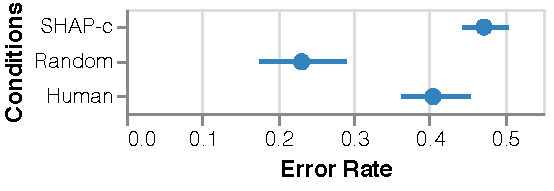
\includegraphics[width=1\columnwidth]{figures/exp_err_rate}
\vspace{-15pt}
\caption{
Error rates on counterfactuals in different conditions. The higher the error rate, the more information missed by the participants (\ie and therefore can better complement model interactions and SHAP.)
}
\vspace{-10pt}
\label{fig:err_rate}
\end{figure}

\paragraph{Results.}
As shown in Figure~\ref{fig:err_rate}, participants performed well on Random (error rate $e=23\%\pm7\%$) but poorly on SHAP-c ($47\%\pm 4\%$), showing that while SHAP and model interactions indeed helped experts simulate model behaviors on some counterfactuals, SHAP-c counterfactuals were beyond their mental models, and \emph{would still add value if they were presented as part of the explanation.}

Participants also missed many Human counterfactuals ($40\%\pm 5\%$), though it was expected --- these cases were surprising even to their human creators.
More interestingly, their performance on Human were slightly better than on SHAP-c, indicating that \emph{SHAP-c were at least as surprising as the Human selected abnormal cases.}

More interestingly, their poor performances on the two conditions were for a different reasons: 
%\ie \emph{Missing inspections v.s. Missing bugs within an inspected spots.}
When the participant mis-predict one particular SHAP-c counterfactual $\xp$, \tofix{80\%} of the time, they submitted at least one queries that's related to the counterfactual (\ie $>75\%$ of the changed tokens in $\xp$ were also changed in the query), and the number dropped to \tofix{$62\%$} in Human.
This indicates that, while participants missed many Human counterfactuals for not replicating the inspection spots (and therefore had to ``guess using intuitions''), they were \emph{misled} by their inspections in the SHAP-c case --- ``give the same prediction as the example I tried'', as one subject articulated.
For example, when the model predicted \emph{Duplicate} on their query \exinline{How do you overcome \add{your} emotional attachment?}, it was hard for them to imagine model predicting \emph{Duplicate} on \exinline{How do you overcome \add{this} emotional attachment?} 
In other words, \emph{SHAP-c found more bugs within spots where humans considered inspected, which is a different bug space compared to the human selected abnormality.}

Moreover, in their freeform responses, 3 out of 6 participants mentioned they prioritized perturbing words with high feature weights, which further indicated the importance of selecting \emph{unexpected prediction change} for them.




\subsection{Global / Interactive Explanations}
\label{subsec:global_exp}

Here, we explore more extensive use of perturbation explanations via examples, but defer more sophisticated designs and evaluations to future work.

\paragraph{Global explanations: impacts of same changes.}
Besides finding abnormal counterfactuals around an individual data point, \emph{global} abnormality provides more systematic observations, and therefore more generalizable model understandings --- yet another important aspect of model explanations~\cite{miller}.
We find \emph{abnormal groups} of counterfactual through two steps: 

First, we group counterfactuals by featurizing them into templates. 
The templates featurization uses the edits between $\xp$ and $x$, like the \tagstr (\fexptag{negation} for the example in Figure~\ref{fig:blank}), the combined templates \fexptemp{\swap{kids}{children}}, etc.
%(1) its \tagstr (\fexptag{negation} for the example in Figure~\ref{fig:blank}), 
%(2) its remove phrases \fexpfrom{kids}, 
%(3) its added phrases \fexpto{not}, \fexpto{children}, and 
%(4) the combined template \fexptemp{\swap{kids}{children}}.
Then, we rank the groups $G = \{ \xp_1, \xp_2, ...\}$ using the entropy of the prediction changes for all counterfactuals in a group, \ie the entropy of the prediction tuple $(f(x), f(\xp))$.
Intuitively larger entropies indicate that the perturbation has unstable impact on the predicted label.

For example, when evaluating the \nli RoBERTa model, one abnormal global perturbation is \swap{two}{three} in the hypothesis.
Out of the 253 counterfactuals whose original prediction $f(x)=$ \emph{entailment}, $138$ flipped to \emph{contradiction}, $22$ to \emph{neutral}, yet $93$ remained \emph{entailment}, resulting in entropy $I=0.91$.
We observe that most cases flipped to \emph{contradiction} have the explicit word ``two'' in the premise, whereas the prediction-intact ones suggest that the model cannot process actual counting.

\ebox{
\textbf{P}: Two women having drinks at the bar.\\
\textbf{H}: \swap{Two}{Three} women are at a bar.\\
\textbf{Pr}: \swap{entailment}{contradiction}\\
--\\
\textbf{P}: A boy and a girl gaze in a clothing store window.\\
\textbf{H}: \swap{Two}{Three} kids are looking in a store window.
\textbf{Pr}: \swap{entailment}{entailment}
}

\begin{comment}
The featurization uses the edits between $\xp$ and $x$: 
(1) its \tagstr (\fexptag{negation} for the example in Figure~\ref{fig:blank}), 
(2) its remove phrases \fexpfrom{kids}, 
(3) its added phrases \fexpto{not}, \fexpto{children}, and 
(4) the combined template \fexptemp{\swap{kids}{children}}.
%For tokens involving multiple changes, we featurize both the primary and the combined changes, and so the example in Figure~\ref{fig:blank} also have additional features like \texttt{\fexptag{negation} \& \fexptag{lexical}}.

For each feature $h$ we compute the its prediction change rate over all the perturbations $\xp \in \xset_{h}$ that have the said feature: 
$R_h = \sum {\mathbb{1}[f(x) \not\eq f(\xp)]} / |\xset_h|$.

Filters on the change rate then reveal different model prediction patterns.\footnote{Because different \nli labels follow very flip patterns, we only include $f(x)=entailment$ examples here}

\noindent\textbf{Mastered patterns.}
Patterns with very high or low change rates (\eg $|R_h-0.5| > \gamma=0.3$) reveal patterns that the model has firmly learned.
In \nli, it includes \fexptemp{\swap{men}{women}} ($R_h=97\%$), \fexptemp{\swap{outdoor}{outside}} ($R_h=0\%$).

\noindent\textbf{Outliers.}
Inspecting the abnormal cases in \emph{mastered patterns}, we find harder to notice examples.
\fexptemp{\swap{three}{four}} changes the 80\% prediction(on 56 changed examples), but all the cases with affected predictions have the explicit pattern ``three'' in the premise, whereas the prediction intact ones show that the model has a hard time processing the actual counting.

\ebox{
\textbf{P}: Three girls fell on top of one another and are laughing.\\
\textbf{H}: \swap{Three}{Four} girls falling and laughing.\\
\textbf{Pr}: \swap{entailment}{contradiction}\\

\textbf{P}: Two little girls and one little boy are running.\\
\textbf{H}: \swap{Three}{Four} kids are running. \\
\textbf{Pr}: \swap{entailment}{entailment}
}

\noindent\textbf{Missed patterns.}
In contrast of the mastered cases, patterns with mild change rates (\eg $|R_h-0.5| < \gamma=0.2$) reveal patterns that the model handles unstably.
For example, the model does not handle the shuffled phrases, echoing the results from \citet{mccoy2019right}.

\ebox{
\fexptag{shuffle}, $R=0.63$ (164 cases)\\
\textbf{P}: The bride in the white dress is surrounded by the groomsmen and bridesmaids, all in black.\\
\textbf{H}: \add{white} woman \remove{in white} is surrounded by others.\\
\textbf{Pr}: \swap{entailment}{entailment}\\

%\textbf{Premise}: Man juggling apples while sitting on a couch with another man on one side and a woman on the other.\\
%\textbf{Hypothesis}: Two \swap{men}{women} sitting near a \swap{woman}{man}.
%\textbf{Prediction}: \swap{entailment}{entailment}\\

\textbf{P}: A man in a wheelchair is being pushed towards a monk.\\
\textbf{H}: The \swap{person is disabled and}{holy person} is being moved towards a \swap{holy}{disabled} person. \\
\textbf{Pr}: \swap{entailment}{entailment}
}

\end{comment}

\paragraph{Interactive explanation.}
Besides automatically selected explanations, users should be allowed to specify a foil, in which case they are implicitly pointing towards the part of the model they do not understand~\cite{miller}.
%Furthermore, the method should allow explanations as a dialog. 
The targeted generation seamlessly support such interactive explanation (ideally in a visual interface), and multi-step drill downs.
In the example: 

\ebox{
\textbf{P}: Some dogs are running on a deserted beach.\\
\textbf{H}: There is only one dog at the beach.\\
\textbf{Pr}: contradiction
}

To understand whether the model responses to quantifiers, an analyst can blank ``only one'', which would reveal that the model predicts entailment correct for both perturbed hypotheses:

\ebox{
\textbf{H}: There \swap{is only one dog}{are multiple dogs} at the beach.\\
\textbf{H}: There is \swap{only}{more than} one dog at the beach.
}

Then, the analyst can keep ``more than one dog'' to inspect how the model react to other changes. 
With the model maintaining entailment on the following examples, the analyst would conclude that there may be a strong correlation between NNS and ``more than one,'' that it overwrites many of the prep constraints.

\ebox{
\textbf{H}: There is \emph{more than} one dog at the beach \add{lying down}.\\
\textbf{H}: There is \emph{more than} one dog at the beach \add{inside a cup}.\\
\textbf{H}: There is \emph{more than} one dog at the beach \add{standing}.
}

